\section{ASPに基づくCAFE問題ソルバー}

開発したCAFE問題ソルバーの構成を図\ref{fig:system}に示す.
CAFE問題ソルバーでは,OVMで表現されたCAFE問題のインスタンスを
ASPファクト形式に変換した後,CAFE問題の制約のASP符号化と結合し,
高速ASPソルバーを用いて解を求める.

本節では,インスタンスのASPファクト形式による表現方法を説明し,
制約の基本的なASP符号化と,その問題点を改良した符号化を提案する.
さらに,優先度付きの目的関数の追加を行うことで,
CAFE問題ソルバーの拡張性の高さを紹介する.
%以降では前者を基本符号化,後者を改良符号化と呼ぶ.

\begin{figure}[tb]
 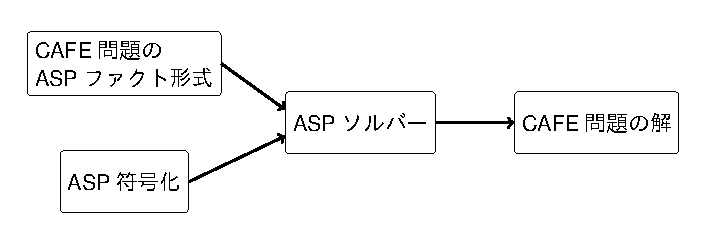
\includegraphics [width=\linewidth]{images/system.eps}
 \caption{CAFE問題ソルバーのシステム概要}
 \label{fig:system}
\end{figure}

\subsection{インスタンスのASPファクト形式}
\lstinputlisting[float=tb,caption={%
インスタンスのASPファクト表現(一部)},%
captionpos=b,frame=single,label=code:ovm2.lp,%
numbers=left,%
breaklines=true,%
columns=fullflexible,keepspaces=true,%
xrightmargin=0zw,% 
xleftmargin=3zw,% 
basicstyle=\ttfamily\scriptsize]{codes/ovm2.lp} 

コード\ref{code:ovm2.lp}は,図\ref{fig:ovm_example}のCAFE問題の
インスタンスの一部をASPファクト形式で表現したものである.

1行目ではタイプ\code{Drive\_Type}を定義している.
2, 3行目ではオプション\code{2WD}と\code{4WD}を定義しており,
どちらもタイプ\code{Drive\_Type}に付随するオプションで,
IWRはそれぞれ\code{125}, \code{200}であることを表している.
5行目ではタイプ\code{Drive_Type}が必須であることを表している.
7行目はオプション\code{STD}がオプション\code{16_inch_Tire}を要求することを,
8行目はオプション\code{V4}がオプション\code{10AT}を排除することを意味する.
このインスタンスでは10行目で装備仕様のグループを3種類求めるように指定しており,
12〜14行目でそれぞれのグループでタイプ\code{Grade}が
\code{STD, DX, LX}に分かれるように初期設定をしている.

装備仕様の燃費と販売台数を示すテーブルも,ASPのファクトとして表現できる.
コード\ref{code:tableFE.lp}, \ref{code:tableSV.lp}にて,各テーブルの一部を示す.
ファクト\code{fe\_map(S,FE)}, \code{sv\_map(S,SV)}は,
装備仕様のIWRの和がSであるとき,燃費と販売台数がFEとSVであることを示している.
例えば,装備仕様のIWRの和が900であるとき,コード\ref{code:tableFE.lp}の1行目は
燃費は11.1km/Lであることを表し,コード\ref{code:tableSV.lp}の1行目は
予想される販売台数が97台であることを表している.ASPでは整数しか扱えないため,
燃費の値は10倍にして記述している.
また,本発表で扱う販売台数のテーブルはIWRの和が5の倍数であるもののみで
構成されているため,販売台数を求めるときにIWRの和の端数を丸める必要がある.

\lstinputlisting[float=tb,caption={%
燃費を算出するテーブルのASPファクト表現},%
captionpos=b,frame=single,label=code:tableFE.lp,%
numbers=left,%
breaklines=true,%
columns=fullflexible,keepspaces=true,%
xrightmargin=0zw,% 
xleftmargin=3zw,% 
basicstyle=\ttfamily\scriptsize]{codes/tableFE.lp} 

\lstinputlisting[float=tb,caption={%
販売台数を算出するテーブルのASPファクト表現},%
captionpos=b,frame=single,label=code:tableSV.lp,%
numbers=left,%
breaklines=true,%
columns=fullflexible,keepspaces=true,%
xrightmargin=0zw,% 
xleftmargin=3zw,% 
basicstyle=\ttfamily\scriptsize]{codes/tableSV.lp} 

\subsection{基本符号化}
\lstinputlisting[float=tb,caption={%
CAFE問題のASP符号化},%
captionpos=b,frame=single,label=code:basic1.lp,%
numbers=left,%
breaklines=true,%
columns=fullflexible,keepspaces=true,%
xrightmargin=0zw,% 
xleftmargin=3zw,% 
basicstyle=\ttfamily\scriptsize]{codes/basic1.lp} 

コード\ref{code:basic1.lp}にCAFE問題の制約のASP符号化(基本符号化)を示す.
2行目は,CAFE基準値として変数\code{t}に整数90を代入している.変数\code{t}の値は
ソルバー使用時にオプションを加えることで,任意の値に変更することができる.

アトム\code{vp(VP,G)}, \code{v(V,G)}は,グループ\code{G}で
それぞれタイプ\code{VP},オプション\code{V}が装備されることを意味する.
%
4行目は,任意のタイプ\code{VP},任意のグループ\code{G}に対してタイプの解候補となる
\code{vp(VP,G)}を導入し,個数制約を用いてグループ\code{G}がタイプ\code{VP}を
装備するか否かの選択をするということを表している.
%
5行目は,一貫性制約を用いて必須であるタイプはすべてのグループで
必ず装備しなければならないという制約を表している.
%
6行目は,グループ\code{G}でタイプ\code{VP}が装備されるとき,
オプションの解候補となる\code{v(V,G)}を導入し,
個数制約を用いてタイプ\code{VP}に付随するオプションの中で
装備するオプションの数をちょうど1つに制限している.


9〜12行目は燃費制約を表している.
9行目は重み付き個数制約を用いて,任意のグループ\code{G}に対して,
装備されるオプション\code{V}の\code{IWR}の和を変数\code{S}に代入し
アトム\code{iwr(S,G)}を生成する.このアトム\code{iwr(S,G)}は,
グループ\code{G}の装備仕様のIWRの和が\code{S}であることを表している.
%
10行目は,任意のグループ\code{G}と任意のIWRの和\code{S},任意の燃費\code{FE}に対して,
\code{iwr(S,G)}かつ\code{fe\_map(S,FE)}ならばアトム\code{fe(FE,G)}を生成する.
このアトム\code{fe(FE,G)}は,グループ\code{G}の装備仕様の燃費が値\code{FE}
であることを表している.
%
11行目は,同様にしてグループ\code{G}の装備仕様の予想販売台数が\code{SV}であることを
表すアトム\code{sv(SV,G)}を生成する.ただし,本研究で扱う販売台数のテーブルは
IWRの和が5の倍数であるもののみで構成されているため,
グループ\code{G}のIWRの和\code{S}に最も近い5の倍数の値\code{S1}を
求める計算を加えている.
%
12行目は,「販売台数を加味した全体の平均燃費が基準値\code{t}以上でなければならない」
という燃費制約を表している.第2節の燃費制約の式を変形すると,以下のようになる.
\\
\begin{displaymath}
 (FE_{1} - t) \times SV_{1} + (FE_{2} - t) \times SV_{2} + (FE_{3} - t)
 \times SV_{3} \geq 0
\end{displaymath}
\\
つまり,すべてのグループの\code{(FE - t)*SV}の和が0以上でなければならないという制約を,
一貫性制約と重み付き個数制約を用いて燃費制約を表現している.

15〜18行目は一貫性制約を用いて要求制約を表している.
15行目は,任意のオプション\code{V},任意のグループ\code{G}に対して,
\code{require\_v\_v(V1,V2)}かつ\code{v(V1,G)}ならば,アトム\code{v(V2,G)}は
真であることを意味する.
16〜18行目は,同様にして,タイプによるオプションの要求,オプションによるタイプの要求,
タイプによるタイプの要求を記述している.OVMの定義にはVPによるVの要求は含まれないが,
CAFE問題では追加して扱うものとする.
21〜24行目は同様にして排除制約を表している.

27行目は一貫性制約を用いて,グループ\code{G}で初期設定として装備することが決められている
\code{V}が選択されなければならないことを表している.

30行目は,目的関数である全体の販売台数の最大化を行っている.




\subsection{ASP符号化の改良}
\lstinputlisting[float=tb,caption={%
改良符号化の一部},%
captionpos=b,frame=single,label=code:basic2.lp,%
numbers=left,%
breaklines=true,%
columns=fullflexible,keepspaces=true,%
xrightmargin=0zw,% 
xleftmargin=3zw,% 
basicstyle=\ttfamily\scriptsize]{codes/basic2.lp} 

コード\ref{code:basic1.lp}の基本符号化では,9行目のIWRの和の候補の生成時に
オプションの個数制約を考慮しておらず,ASPソルバーでの基礎化の際に,
一つもオプションを選択しない場合やすべてのオプションを選択した場合など,
明らかに成立しないオプションの選択の仕方によるIWRの和まで解の候補として生成してしまう.
そこで,IWRの和の上下限をより厳密に制限することで基礎化によって生成される
ルール数を減らし,探索空間の削減を行う改良符号化を考案した.
改良符号化では,IWRの和の上限をすべてのタイプでIWRが最大のオプションを選択した場合の和,
下限を必須であるタイプのみでIWRが最小のオプションを選択した場合の和とする.
改良符号化の一部をコード\ref{code:basic2.lp}に示す.
改良符号化は,コード\ref{code:basic1.lp}の9行目を
コード\ref{code:basic2.lp}に置き換えたものである.

コード\ref{code:basic2.lp}の2〜5行目で前処理としてIWRの和の上下限の計算を行う.
2行目では,すべてのタイプ\code{VP}についてそれに付随するオプションの中で最大の
IWRを\code{UB}として,アトム\code{ub_vp(UB,VP)}を生成する.
3行目では,すべてのタイプの\code{UB}の和を求め,IWRの和の上限を表すアトム
\code{ub_iwr(S)}を生成している.
4行目では同様に,すべてのタイプについて最小のIWRを\code{LB}として,
アトム\code{lb_vp(LB,VP)}を生成する.
5行目では,必須であるタイプのみの\code{LB}の和を求め,IWRの和の下限を表すアトム
\code{lb_iwr(S)}を生成している.
8行目では,この上下限の値でIWRの和の候補を求める範囲を制限している.

\subsection{ASP符号化の拡張}
CAFE問題ソルバーでは,販売台数の等しい解が複数存在するとき,
目的関数を追加することで解に優劣をつけることができる.
新たな目的関数として,オプション数の最小化を考える.
これは,製造ラインの削減や大量生産を可能にして製造の効率化を狙うためである.
コード\ref{code:basic1.lp}の30行目をコード\ref{code:obj_op.lp}に置き換えることで
オプション数最小化を実現可能である.
コード\ref{code:obj_op.lp}の5行目では,いずれかのグループで選択された
オプション\code{V}を\code{used_v(V)}で表し,6行目でこのアトムの数を
最小化することでオプション数最小化を表現している.
優先度は販売台数最大化,オプション数最小化の順で,
販売台数の等しい複数の解候補が存在するとき最もオプション数が少ないものを解とする.

このように,ASPを用いたCAFE問題ソルバーでは容易に問題を拡張できる.

\lstinputlisting[float=tb,caption={%
オプション数最小化},%
captionpos=b,frame=single,label=code:obj_op.lp,%
numbers=left,%
breaklines=true,%
columns=fullflexible,keepspaces=true,%
xrightmargin=0zw,% 
xleftmargin=3zw,% 
basicstyle=\ttfamily\scriptsize]{codes/obj_op.lp} 
